\subsection*{Stop, Question, and Frisk data}
\subsubsection*{Background}
Since x the stop, question, and frisk practice is implemented in New York City. A police officer is allowed to stop a person if they have reasonable suspicion that the person has committed, is committing, or is about to commit a crime.
During the stop the officer is allowed to frisk a person (pat-down the person's outer clothing) or search them more carefully.
The stop can result in a summon, an arrest or no further consequences. After a stop was made, the officer is required to fill out a form, documenting the stop. This data is published yearly by the NYPD.
Many citizens have critisised the stop and frisk practice. There is disagreement about whether the strategy is effective in reducing the crime rates of the city. The police has been repeatedly critisised for over-targetting people of colour.
Stop and Frisk practice during 2004 to 2012 has been deemed as unconstitutional. {\color{red} source}

\subsubsection*{Data description}
The raw dataset consists of 16971 observations and 82 variables. We first discarded all the variables that have more than 20\% missing values.
34 variables remain that provide us with information about the stop and demographic information of the stopped person. From this reduced dataset we filter out the complete cases and end up with 12039 observations.
Simply discarding the missing values and only training on complete cases is discouraged by \cite{fernando2021}. We opt for this approach regardless, since imputation of the missing values is not straight forward
but treating missing values as an extra category (which some random forest learners in mlr3 can do) will introduce complications when we implement some fairness methods later on.
(many fairness methods can not deal with missing data, especially in the protected attribute, which makes sense, since they base their decision on it). 
Figure x {\color{red}{combine the two race distribution by borough plots}} shows that consistently across all five boroughs black people are stopped most often, eventhough they do not make up the largest ethinic group in any of the boroughs. White people, on the other hand, are relatively speaking underrepresented in the data.


% arrestment rates between PA groups
For the study of a fair algorithm, we focus our attention on arrestment rates between different ethnic groups.
The arrestment rate of PoC is lower than for white people. This is a first indicator for how difficult it can be to measure fairness through observational metrics. Do higher arrestment rates among white people indicate that white people are more easily arrested, indicating discrimination against white people? Or do the lower arrestment rates for PoC reflect that police officers stop PoC more leniently, thus leading to many innocent PoC being stopped?
When we compare the race distribution of NYC to the race distribution in the SQF data, it is clear that in terms of race the SQF data does not represent the general population of the city.
% borough specific graphics?

\textbf{Fairness Auditing}
% insert a graphic
\begin{figure}
    \centering
    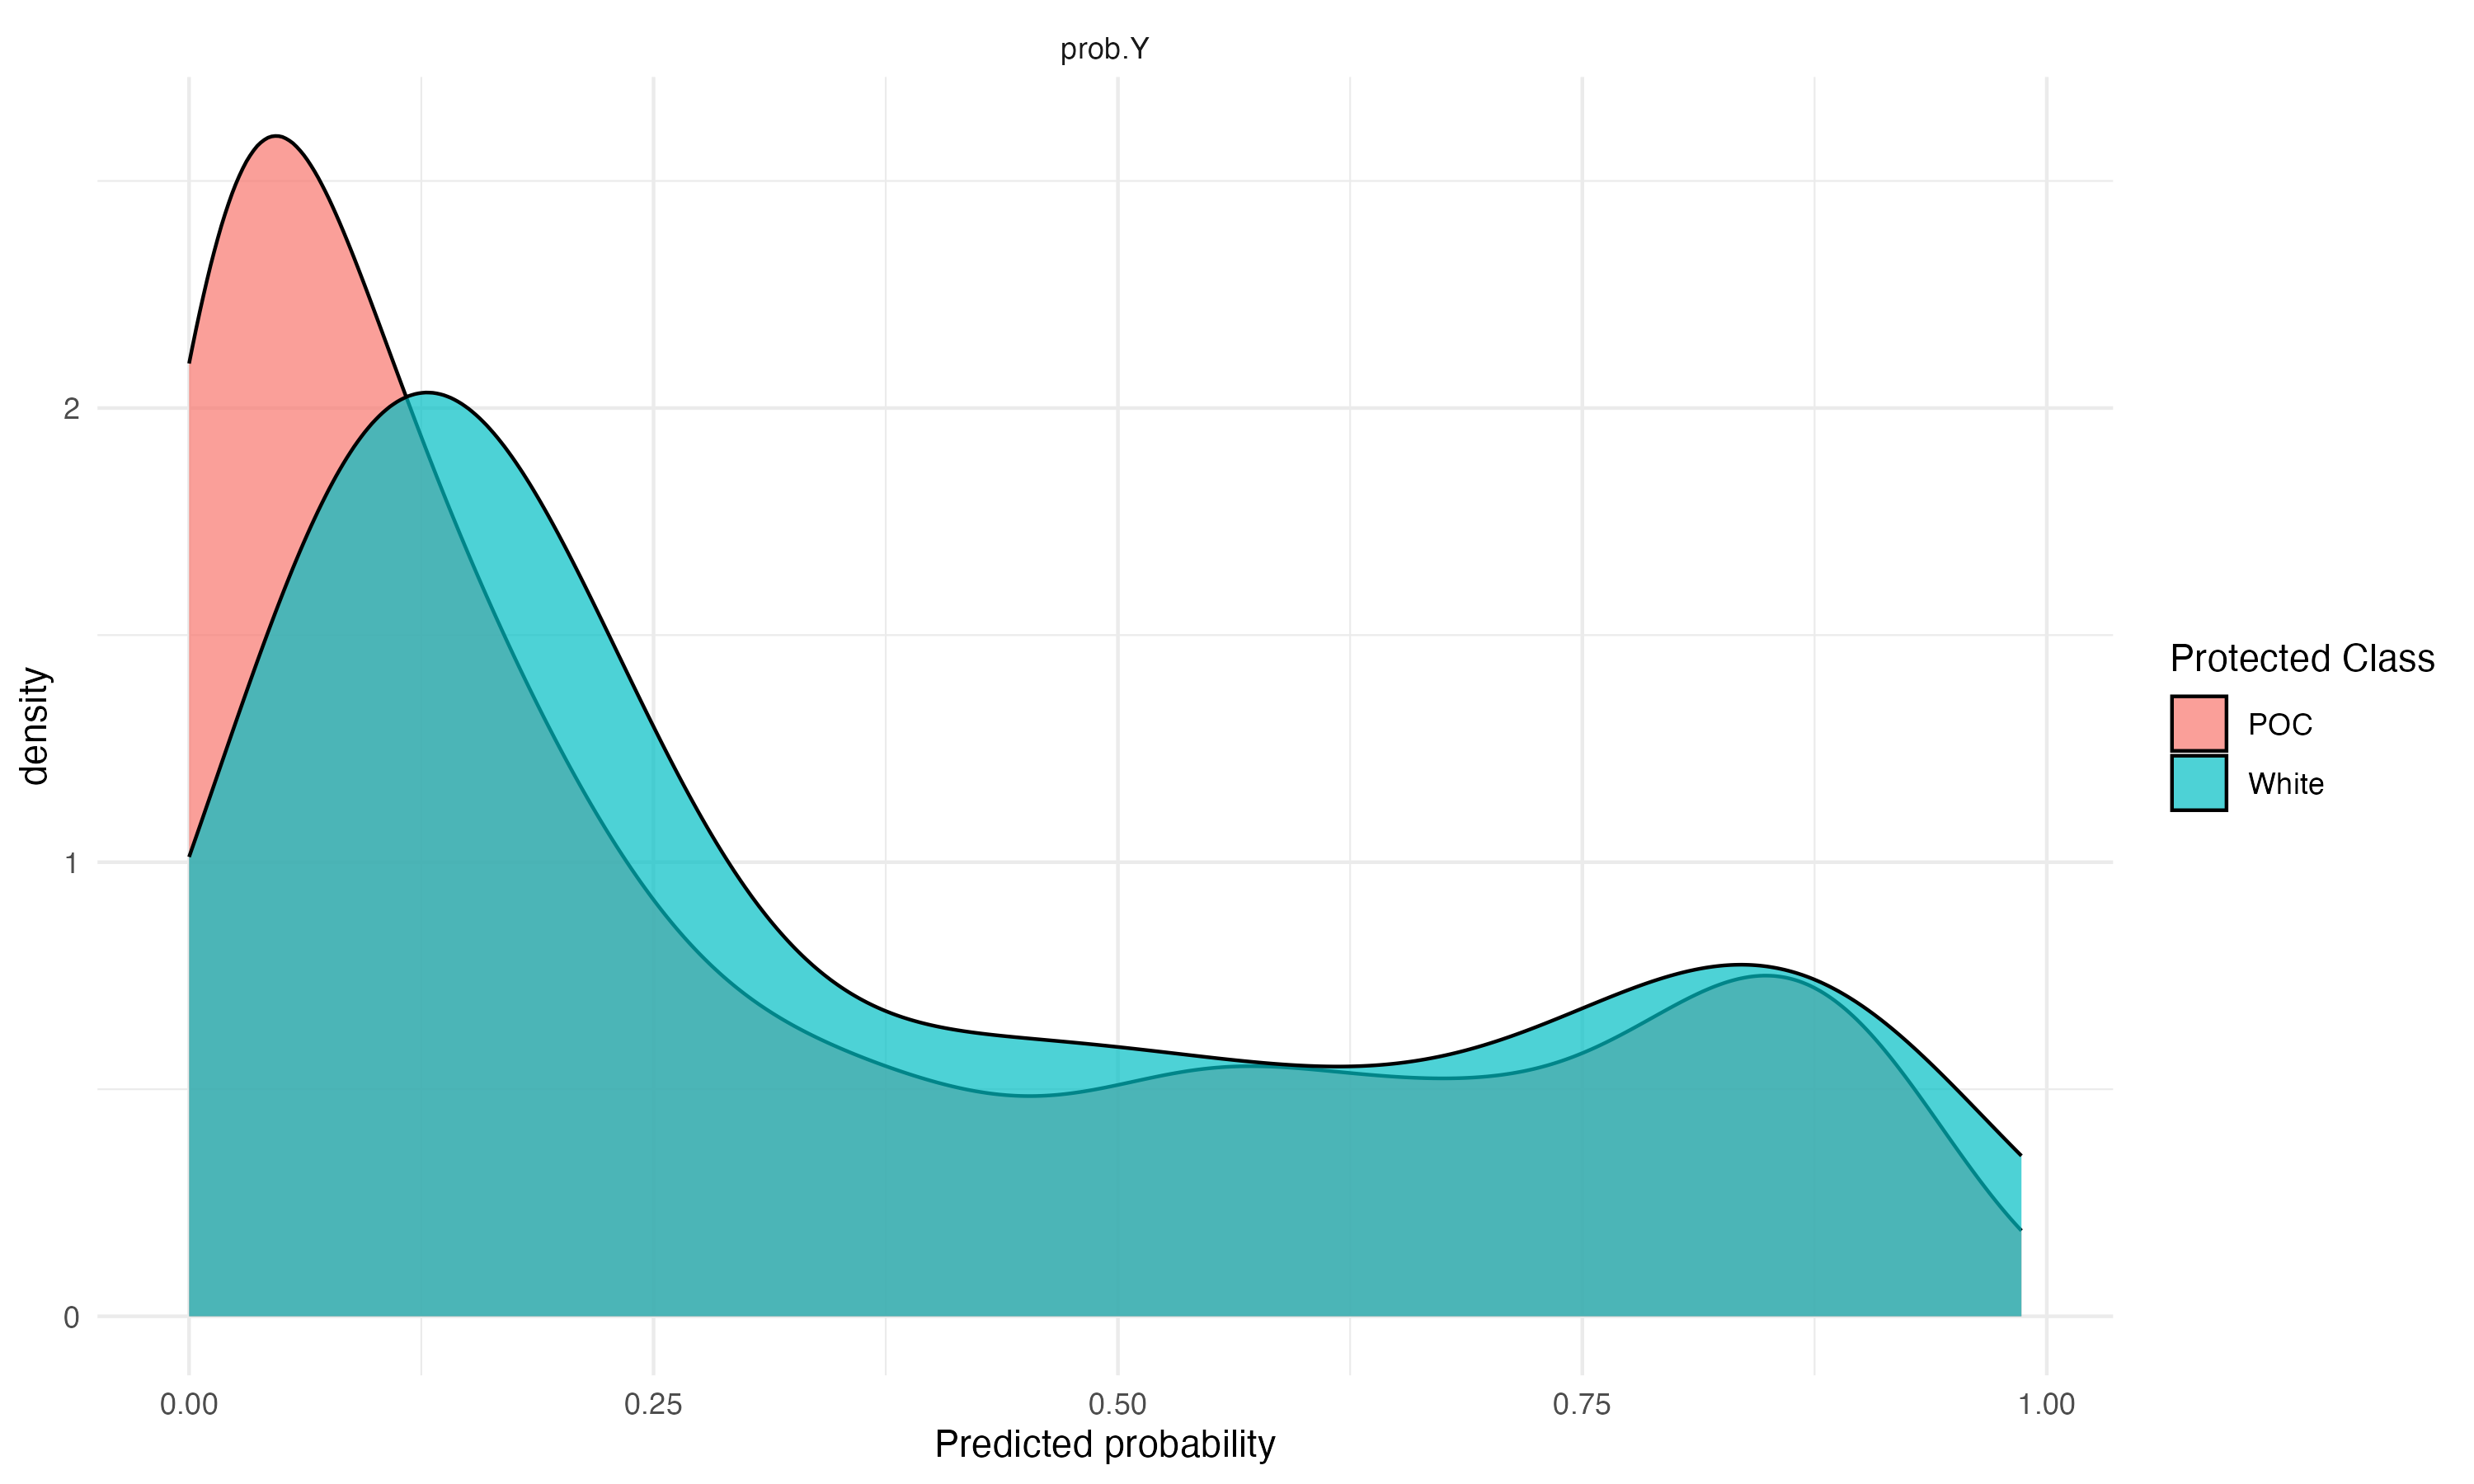
\includegraphics[width=0.7\textwidth]{../figures/sqf_case_study_plot1.png}
    \caption{Density of predicted probabilities both groups.}
    \label{fig:fairness_density}
\end{figure}
We want to train a binary classifier on the SQF data that predicts the arrestment of a person. To adjust our situation to the common binary classification, binary PA scenario in the fairness literature, we
dichotomise the race attribute by grouping "Black", "Black Hispanic", and "White Hispanic" into the "PoC" group and "White", "Asian Pacific", etc. into the "White" group. \footnote{This, of course, is an oversimplification of the scenario and we know that this grouping can be critisised from a social science standpoint. We see this as a compromise to keep things straight forward. more nuanced scenarios can be addressed in future work.} 
We train a regular random forest and make a fairness audit, measuring fairness with various group metrics implemented in mlr3fairness.
Measured by these group metrics the random forest classifier is already relatively fair. There are minor differences between groups, but exact equality cannot be expected in practice, thus it is common to allow for a certain margin of error.
Especially the error rates (fnr, fpr) are very similar between groups, thus Separation seems to be satisfied overall. Sufficiency metrics have larger differences, though they are still minor. From \autoref{fig:fairness_metrics_barplot} we can directly see that the the positive predictive value has a relatively large difference between groups, while the false positive rate is basically the same between groups. Also the accuracy is very similar.

\begin{figure}
    \centering
    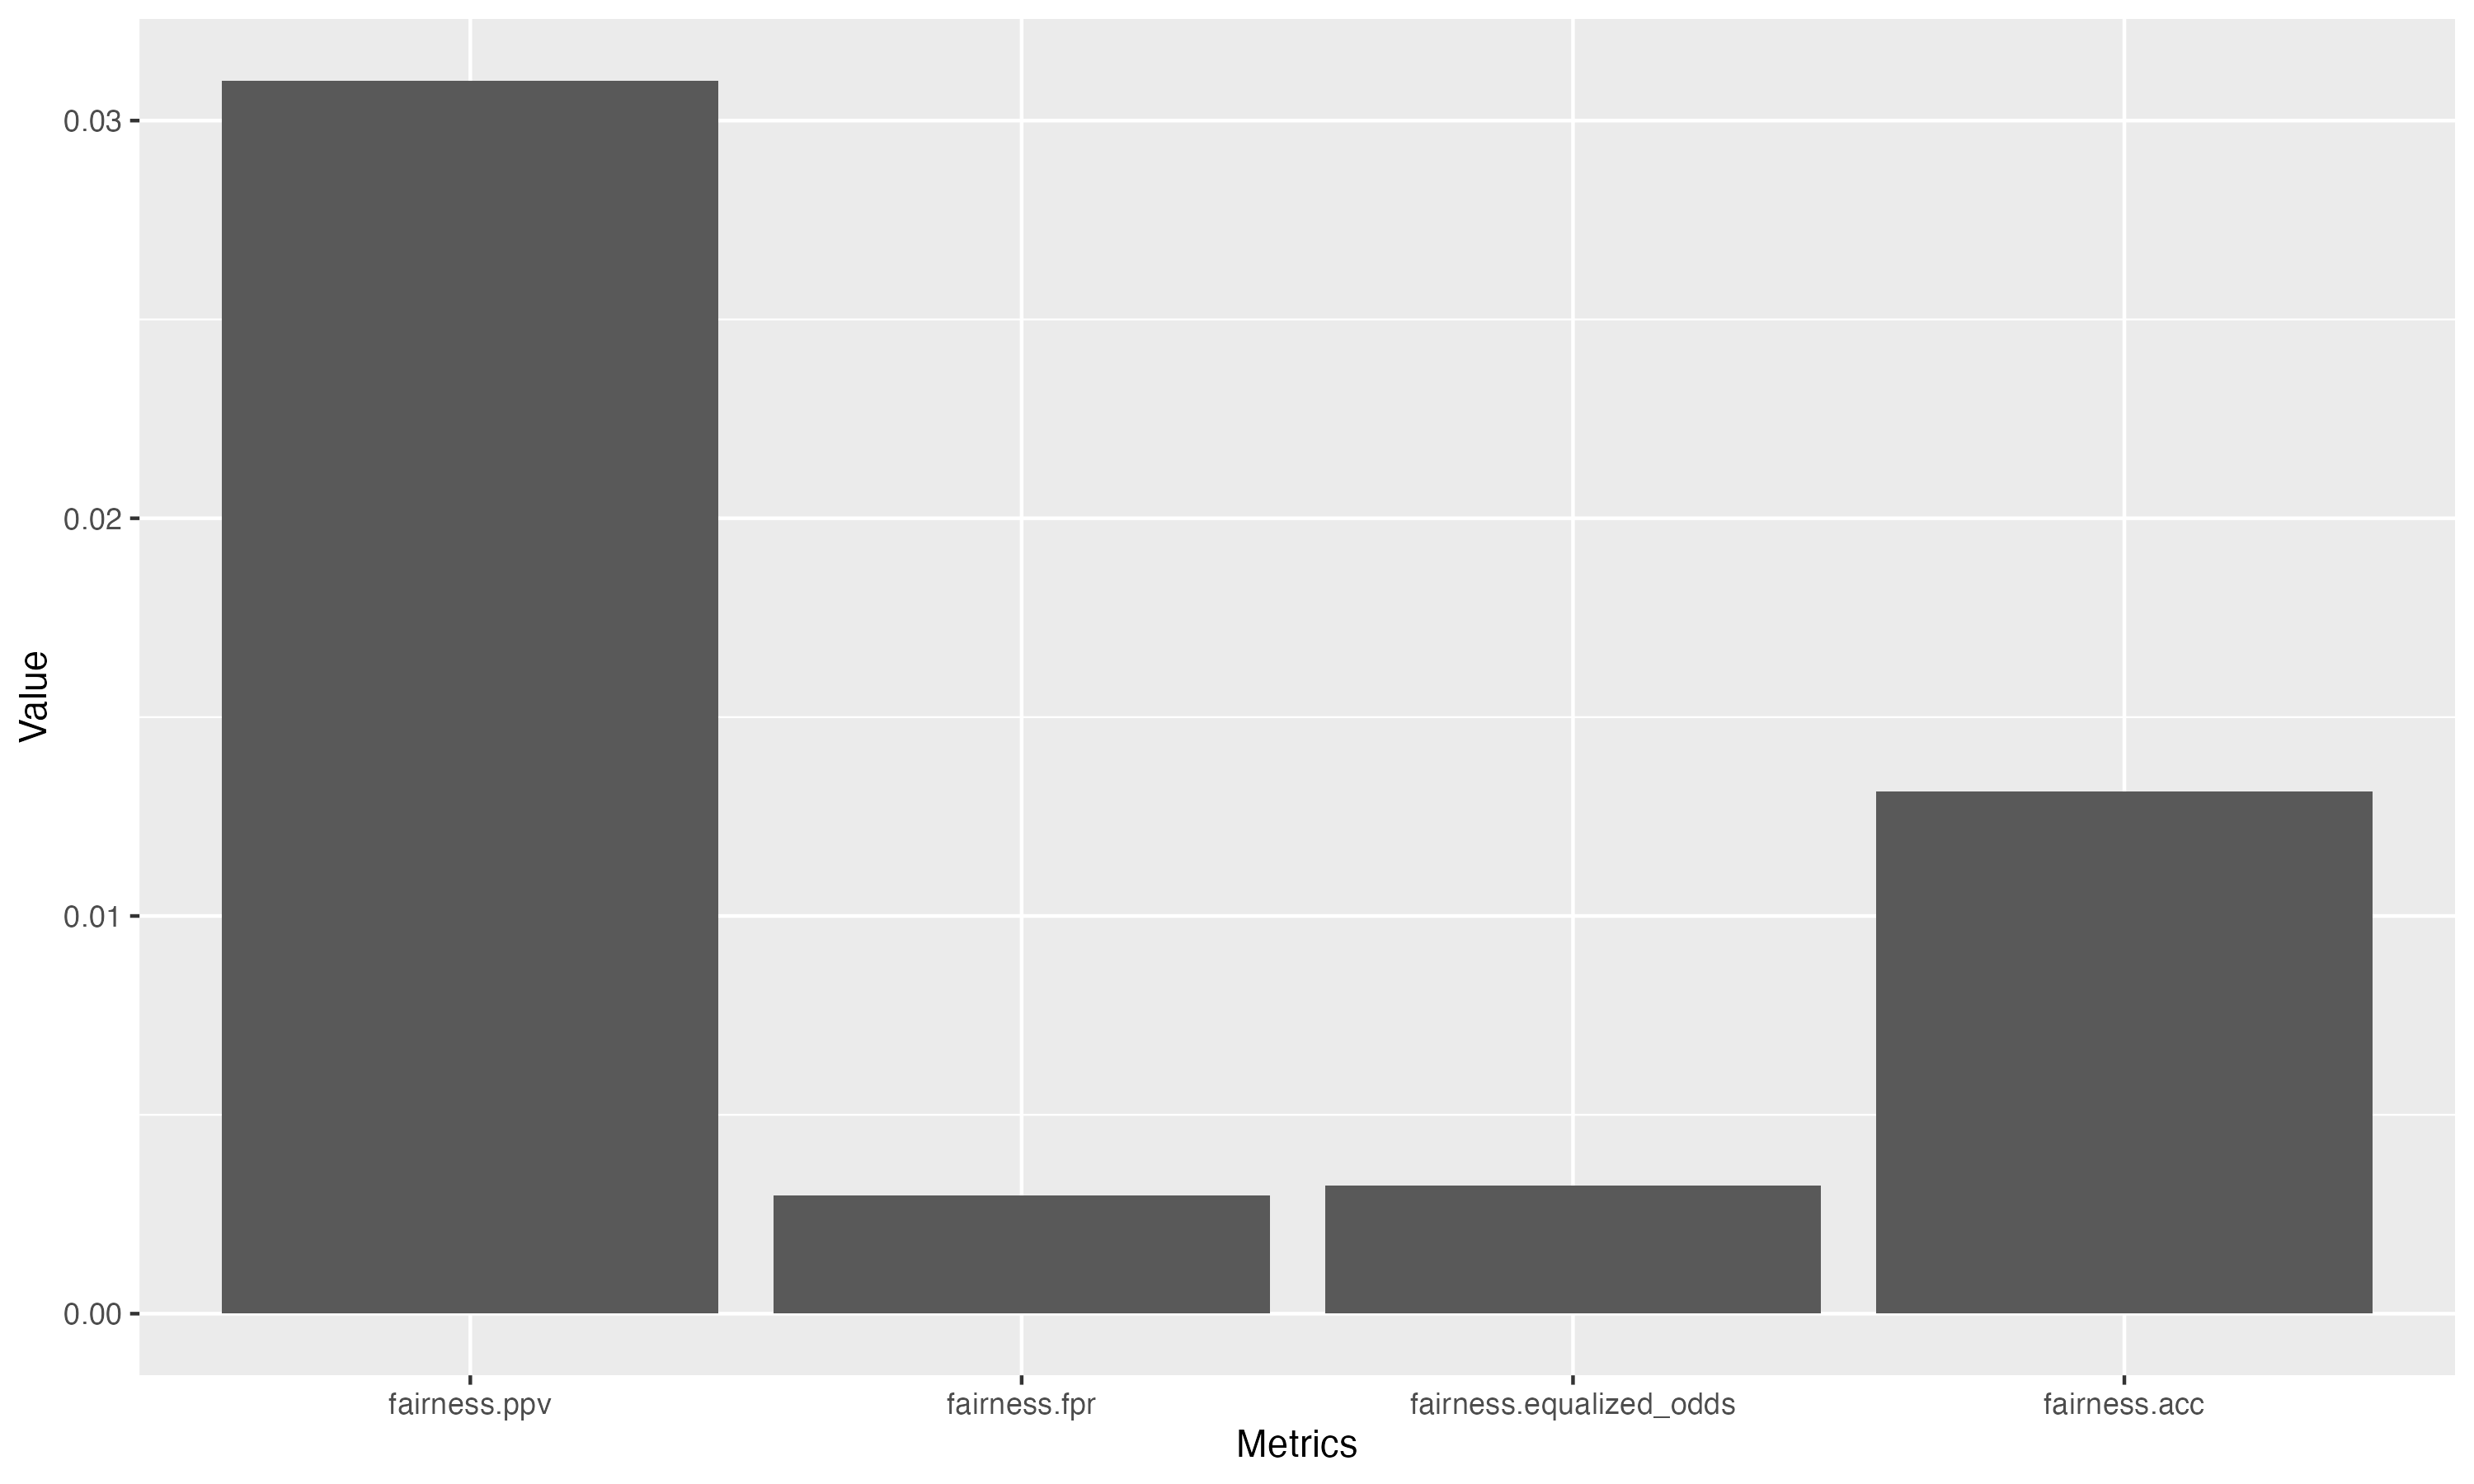
\includegraphics[width=0.7\textwidth]{../figures/sqf_case_study_plot2.png}
    \caption{Comparison of fairness metrics.}
    \label{fig:fairness_metrics_barplot}
\end{figure}

\textbf{Fairness Experiment}
% - fairness metrics (table) for dichotomised race and for full race grouping in appendix.
% - fairness methods (inspired by the article)

% Reweighing: https://mlr3fairness.mlr-org.com/reference/mlr_pipeops_reweighing.html?utm_source=chatgpt.com#format
% Fair logistic regression: https://rdrr.io/cran/mlr3fairness/man/mlr_learners_classif.fairzlrm.html?utm_source=chatgpt.com
% EOd: https://mlr3fairness.mlr-org.com/reference/mlr_pipeops_equalized_odds.html?utm_source=chatgpt.com
% mlr3book: https://mlr3book.mlr-org.com/chapters/chapter14/algorithmic_fairness.html?utm_source=chatgpt.com#bias-and-fairness
% https://mlr3fairness.mlr-org.com/#debiasing-methods

Despite the algorithm being already really fair according to group metrics, we want to examine the effect of different fairness methods.
mlr3fairness currently has two preprocessing methods, one postprocessing method and several fairness adjusted models implemented. We decide to use a reweighing methods that works with assigning weights to the observations to equalise the distribution of $P(Y|PA)$.
The inprocessing method is a fairness-adjusted logistic regression implemented in mlr3fairness inspired by Zafar et. al. This method optimises for statistical parity. The postprocessing method we choose aims for equalised odds and it works by randomly flipping a subset of predictions with pre-computed probabilities in order to satisfy equalised odds constraints.
Fig. x plots the classifier's performance (measured by accuracy) on the x-axis and the fairness (measured by ppv) on the y-axis. A classifier that is fair and accurate would be in the bottom right corner.
\begin{figure}
    \centering
    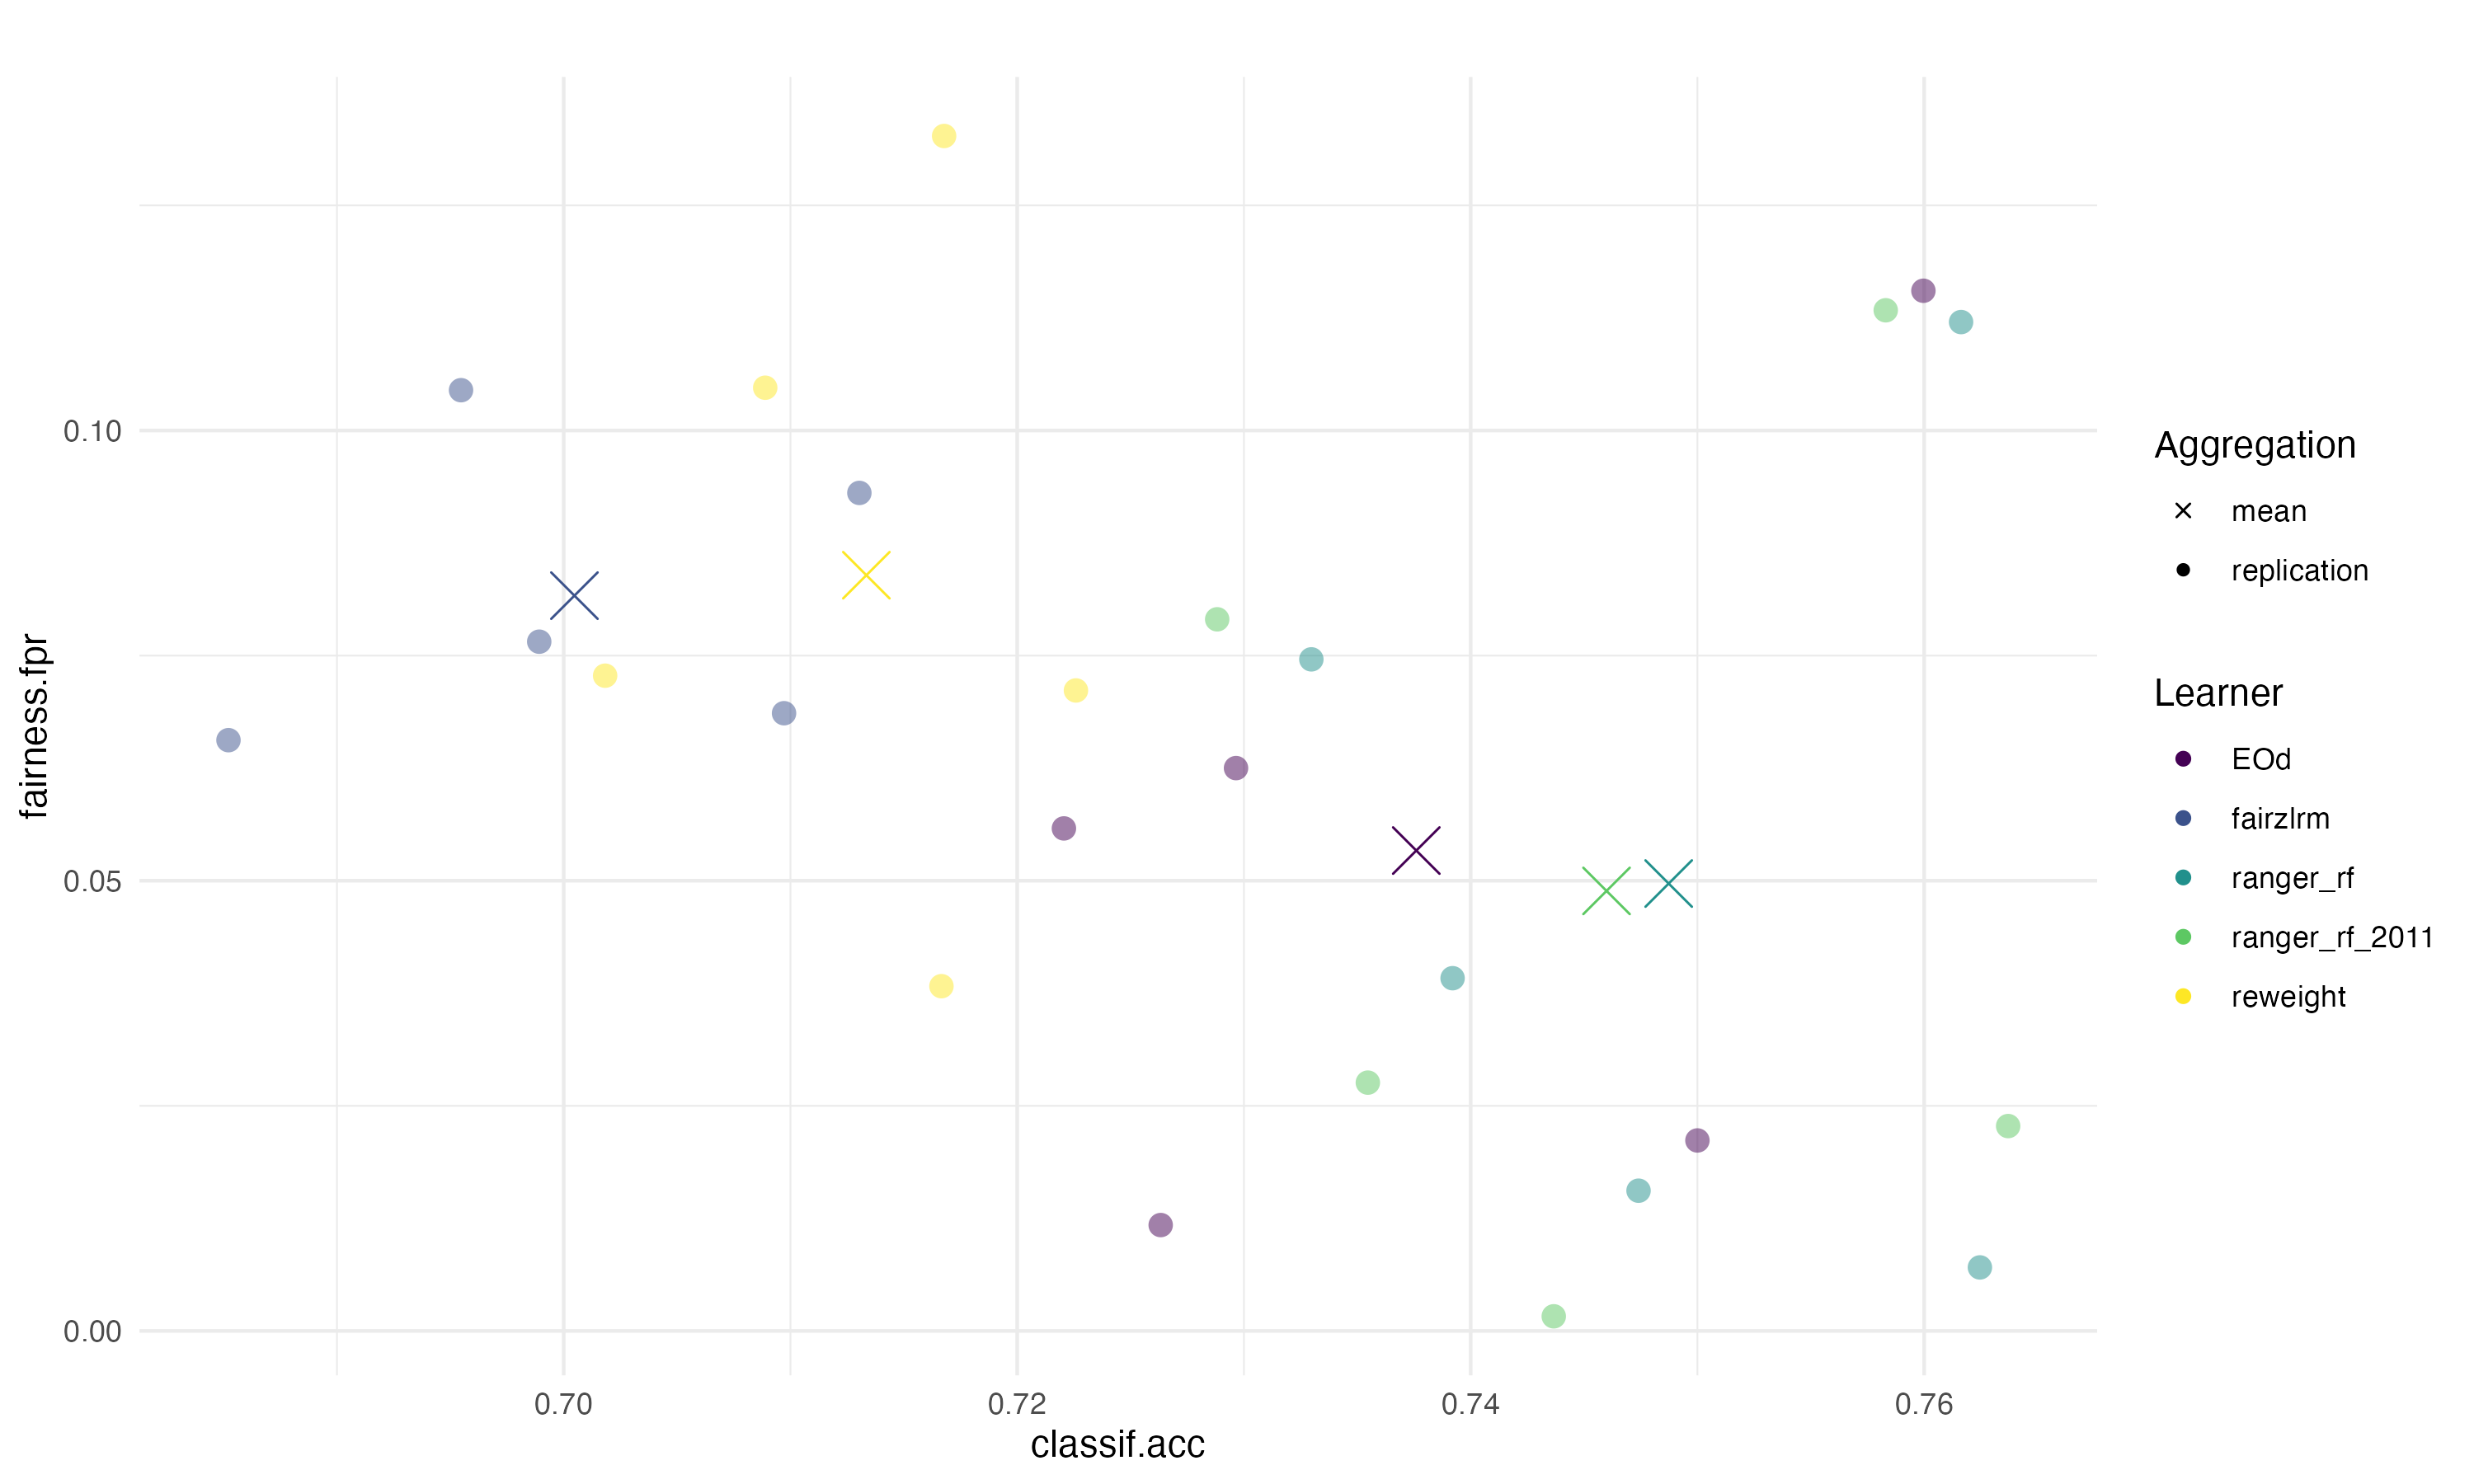
\includegraphics[width=0.7\textwidth]{../figures/sqf_case_study_plot3.png}
    \caption{Performance and fairness of different classifiers.}
    \label{fig:fairness_performance}
\end{figure}
% This all does not really make sense: the classifier performs worst for Sufficiency metrics but the fairness adjustments I make are all for Separtion or Independence


This is all good and insightful, but actually the picture for this data is more complex.
The data introduced three main challenges: selection bias; missing data; class imbalance.

We reviewed paper that address the first of these challenges, since the SQF data is typically used to illustrate this challenge (not the other ones).
% - number of stops conducted but with background information who governed at that time (see Obsidian)
% - transparent explanation of feature selection (similar to Data Transparanecy paper)
% - distribution of race in SQF data vs NYC
% - grouping to black, white, black hispanic, white hispanic, others --> arrestment rates in these groups

